\begin{figure}[H]
	\centering
	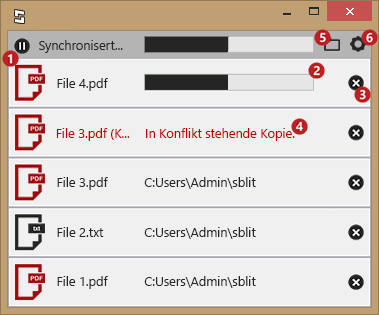
\includegraphics[]{images/systemtray.png}
  \caption{Menüfenster beim Systemtray}
\end{figure}

Mit einem Rechtsklick auf das Icon im System-Tray öffnet sich eine kleine Menüauswahl,
bei der folgende Punkte zur Auswahl stehen:

\begin{description}

	\item[{Configuration}]
		Öffnet das Konfigurationsmenü.

	\item[{Export Key}]
		Öffnet einen Dialog zur Auswahl des Speicherorts. In der exportieren Text-Datei befindet
		sich der öffentliche Schlüssel des eigenen Gerätes und der symmetrische Schlüssel für
		alle \gls{syncpartner}.

	\item[{Shutdown sblit}]
	  Stoppt alle laufenden Synchronisationen und beendet die Anwendung.
\end{description}
